\chapter{Explaining Algorithm Performance Distributions Through Interpretable Statistics}
\label{sec:dist_explain}

% Main text
\section{Introduction}
\label{sec:intro}

Empirical performance models (EPMs) are data-driven predictive models that learn the relationship between problem instance features and an algorithm performance metric, such as expected running time or solution quality. They serve as critical components in automated algorithm selection, configuration, and parameter tuning across various domains, including compiler optimisation, database query optimisation, and machine learning.

While traditional EPMs predict a single expected value (typically mean running time), they fail to account for the stochastic nature of modern randomised algorithms. For combinatorial search and optimisation, state-of-the-art solvers rely heavily on randomisation to navigate vast search spaces, resulting in running times that vary substantially across runs on the same instance~\citep{HooStt04}. Consequently, capturing and explaining the full performance distribution—rather than just the mean—is essential for risk-sensitive applications where tail behaviour, failure rates, or consistency guarantees are critical.

To address this, recent approaches such as DistNet~\citep{EggEtAl18} model full per-instance running time distributions. However, these methods are either too compute-intensive or fail to provide explainable insights. Indeed, while EPMs have traditionally been used to analyse algorithm behaviour (see, e.g.,~\citealp{HutEtAl13}), existing explainability techniques are restricted to single-value predictors. This creates a fundamental discrepancy: the algorithms of interest exhibit complex, stochastic distributions, yet their explanations are derived from simplified, deterministic approximations. As a result, critical behaviours like tail risks and performance variance remain opaque.

In this work, we fill this gap. Our contributions are:
(i) We propose explainability measures for distribution predictors by decomposing predicted distributions into interpretable statistics (such as mean, variance, and skewness) and analysing feature effects using permutation importance and individual conditional expectation (ICE) curves.
(ii) We present a tree-based XGBoost approach to performance distribution prediction that matches the accuracy of neural-network-based models while offering substantially lower computational cost.
(iii) We empirically evaluate our approach on SAT solving and automated planning, demonstrating that different instance features govern scale vs. shape statistics, yielding new insights into algorithm behaviour.

\section{Background and related work}
\label{sec:bg}

In this section, we formally define empirical performance models, review existing EPM-based explainability methods, and discuss prior approaches to predicting performance distributions.

\subsection{Empirical performance models}
\label{sec:epm}

Given an algorithm $\mathcal{A}$ that operates on 
% \hh{slightly modified:}
instances $I$ from an instance set $\in\mathcal{I}$, with an associated feature vector $\mathbf{z}_{I}\in\mathcal{F}$ that describes $I$, and a measured performance $p_I\in\mathcal{P}$ (\emph{e.g.}, running time, solution quality or accuracy), an empirical performance model (EPM) is a predictor 
$f: \mathcal{F} \to \mathcal{P}$ %\aj{inline to save space}
% \begin{equation}
%     f: \mathcal{F} \to \mathcal{P}
% \end{equation}
that generalises from a set of observed pairs $\mathcal{D}_\text{train}=\{(\mathbf{z}_{I},p_I) \mid I\in\mathcal{I}_\text{train}\}$ to unseen instances $\mathcal{D}_\text{test}=\{(\mathbf{z}_{I},p_I) \mid I\in\mathcal{I}_\text{test}\}$. 

EPMs have been developed for a wide range of tasks, including automated algorithm selection~\citep{XuEtAl08, Kotthoff2016}, algorithm configuration and parameter tuning~\citep{HutEtAl12, HutEtAl06}, data centre and cloud scheduling~\citep{LeeEtAl25, IslEtAl12, SaxEtAl23, PhaEtAl20}, compiler optimisation~\citep{YotEtAl03, AshEtAl18}, and database query optimisation~\citep{WuEtAl20}. EPMs require a set of features describing instances as an input to the model. For $\mathcal{NP}$-complete problems, high-level properties of instances are encoded to serve as an instance identifier, such as the SATzilla features for propositional satisfiability (SAT)~\citep{HutEtAl14,ShaHoo24} and causal-graph or planning-graph features for automated planning~\citep{FawEtAl14}. 

For stochastic algorithms, the performance of $\mathcal{A}$ on a fixed instance $I$ is a random variable. Traditional EPMs handle this stochasticity by either: (i) modelling an aggregate statistic calculated from repeated runs (e.g., the empirical mean or median), or (ii) training directly on noisy, single-run observations. In both cases, the EPM outputs a single scalar value, discarding all information about the variance and shape of the underlying distribution.


To capture the complete run-to-run variation of stochastic algorithms, \citet{EggEtAl18} introduced \emph{DistNet}, a neural network that predicts the parameters of a per-instance running time distribution (e.g., a log-normal distribution). DistNet is trained by minimising the negative log-likelihood (NLL) of individual run observations, which is more efficient and numerically stable than a two-stage approach that first fits distribution parameters per instance and then regresses on those parameters.

To improve predictive quality in data-scarce regimes, \emph{BayesDistNet}~\citep{TueBur21} replaces the deterministic network with a Bayesian neural network (BNN). During inference, BayesDistNet generates running-time samples by repeatedly evaluating the BNN with different weight samples, subsequently fitting a parametric distribution post-hoc. While effective with few training runs, this sampling-based inference introduces substantial computational overhead. Furthermore, because BNN predictions rely on stochastic weight samples, feature attribution becomes unstable and computationally prohibitive, making it ill-suited for explainability.

\subsection{Explainability of algorithms using EPMs}
To gain insights into why an algorithm performs well or poorly on specific instances, researchers have leveraged EPMs for feature and parameter attribution. For example, \citet{HutEtAl13} used forward selection to identify key parameter-feature interactions, and \citet{HutEtAl14a} proposed functional ANOVA to quantify hyperparameter importance. More recently, model-agnostic explanation tools have been applied to EPMs, such as partial dependence plots (PDP) and individual conditional expectation (ICE) curves to visualise feature effects~\citep{MooEtAl21}, and SHAP interactions to analyse hyperparameter relationships~\citep{WevEtAl25}.

Crucially, all of these techniques assume a scalar-valued prediction target. Because they map features to a single performance value, they cannot be directly applied to models that output full parametric distributions or sample sets.

\section{Explainability of performance distribution predictions}
\label{sec:explainability}

Our EPM predicts the parameters $\boldsymbol\theta$ of a given parametric family (\emph{e.g.,} log-normal or inverse Gaussian) as a function of instance features, \emph{i.e.}, $\boldsymbol\theta=f(\mathbf{z}_I)$. Each summary statistic $s$ is then a function of these parameters, $s=h_s(\boldsymbol\theta)$. 
% \aj{Shouldn't we explicitly define/introduce the hat variants of symbols as estimators of the true values?}
Therefore, we can represent the summary statistic function $g_s$ given instance features $\mathbf{z}_I$ as
% \begin{equation*}
    $g_s(\mathbf{z}_I) = h_s(f(\mathbf{z}_I))$.
To explain the distribution predictions, we analyse how instance features affect the following summary statistics of the predicted distribution: 
\emph{mean:} the expected (average) performance (\emph{e.g.,} running time);
% \hh{should we stick to performance here and in the remainder of Section 3 + 4 and switch to running time in Section 5?}\aj{done}
\emph{variance:} how strongly performance fluctuates around the mean, \emph{i.e.,} overall spread;
\emph{skewness:} the degree to which the distribution is uneven toward unusually small or large performance values;
\emph{kurtosis:} the extent to which  probability mass lies in the tails (which impacts the prevalence of outliers); and
\emph{interquartile range (IQR):} the spread between the $25^{th}$ and $75^{th}$ percentiles, robust to extreme runs.
This representation allows standard model-agnostic explainability tools to be applied per statistic, relating instance features directly to interpretable aspects of the distribution rather than to raw distribution parameters.
In other words, the usage of statistics allows for a higher degree of explainability than simply explaining the outputs of the model.

% \begin{itemize}
%     \item \textbf{Mean:} the expected (average) running time.
%     \item \textbf{Variance:} how strongly running times fluctuate around the mean, \emph{i.e.,} overall spread.
%     \item \textbf{Skewness:} whether the distribution is uneven toward unusually small or large running times.
%     \item \textbf{Kurtosis:} how much probability mass \changed{lies} in the tails (and hence the possibility for outliers).
%     \item \textbf{Interquartile range (IQR):} the spread between the $25^{th}$ and $75^{th}$ percentiles, robust to extreme runs.
% \end{itemize}

% \textbf{Mean:} the expected (average) running time.


% \textbf{Variance:} how strongly running times fluctuate around the mean, \emph{i.e.,} overall spread.


% \textbf{Skewness:} whether the distribution is uneven toward unusually small or large running times.


% \textbf{Kurtosis:} how much probability mass sits in the tails (and hence the possibility for outliers).


% \textbf{Interquartile range (IQR):} the spread between the 25th and 75th percentiles, robust to extreme runs.


% \begin{itemize}
%     \item \textbf{Mean:} the expected (average) running time.
%     \item \textbf{Variance:} how strongly running times fluctuate around the mean, \emph{i.e.,} overall spread.
%     \item \textbf{Skewness:} whether the distribution is uneven toward unusually small or large running times.
%     \item \textbf{Kurtosis:} how much probability mass sits in the tails (and hence the possibility for outliers).
%     \item \textbf{Interquartile range (IQR):} the spread between the 25th and 75th percentiles, robust to extreme runs.
% \end{itemize}
% \hh{the following is very good; if we are pressed for space, IMO, the paragraph before can be condensed into one sentence mentioning the (widely used) summary statistics.}
Together, these five statistics provide a compact and complementary characterisation of a predicted performance distribution: mean captures typical performance (location), variance captures overall uncertainty (scale), skewness and kurtosis describe asymmetry and tail heaviness (possibility for outliers), and the IQR provides a robust spread measure that is less sensitive to extreme runs. 
% Using this low-dimensional set of metrics allows us to apply
% % \aj{allows us to apply} 
% % lets us apply 
% standard, model-agnostic explainability tools to interpretable quantities, rather than attempting to directly attribute effects on the full predicted distribution to instance features.
% \hh{attribute to what? instance features or characteristics?}

Focusing on summary statistics serves two purposes. First, it yields explanations that are directly actionable: for example, practitioners may prefer algorithms whose predicted mean is low \emph{and} whose predicted upper-tail behaviour is mild, even if the average performance is similar. Second, it makes the explanation problem well-posed across different distribution families: regardless of whether we predict a log-normal, inverse Gaussian, or another parametric family, the statistics above provide a common interface for interpretation.

We emphasise that these statistics are not equally easy to estimate from limited data. Mean and IQR tend to be relatively stable even with few runs per instance, whereas higher-order moments (skewness and kurtosis) can be noisy and sensitive to rare extreme runs. In our experiments, we therefore interpret skewness/kurtosis explanations primarily as indicators of changes in tail behaviour rather than precise moment estimates.


\subsection{Permutation importance}
\label{sec:perm_importance}

% Our EPM predicts the parameters $\boldsymbol\theta$ of a given parametric family (\emph{e.g.,} log-normal or inverse Gaussian) as a function of instance features, \emph{i.e.}, $\boldsymbol\theta=f(\mathbf{z}_I)$. Each summary statistic $s$ (such as the mean and variance) is then a function of these parameters, $s=h_s(\boldsymbol\theta)$. 
% % \aj{Shouldn't we explicitly define/introduce the hat variants of symbols as estimators of the true values?}
% Therefore, we can represent the summary statistic function $g_s$ given instance features $\mathbf{z}_I$ as
% % \begin{equation*}
%     $g_s(\mathbf{z}_I) = h_s(f(\mathbf{z}_I))$.
% \end{equation*}


% The first explainability property we look at is feature importance: for each statistic, we would like to know \emph{which features} are the most influential. For this purpose, 
To understand \emph{which features} are the most influential for each statistic, we apply permutation importance~\citep{Breiman2001} to $g_s$. 
For a statistic $s$, we measure predictive accuracy by the mean squared error between the predicted statistic $g_s(\mathbf{z}_I)$ and the corresponding statistic estimated from the observed running time distribution of instance $I$.
The method randomly shuffles the values of one feature across instances, breaking any association between that feature and the statistic-specific target, and measures the resulting increase in MSE: important features yield a substantially larger increase, while irrelevant features cause negligible changes.
% The method operates by randomly shuffling the values of a single feature across observations while keeping all other features fixed, thereby breaking any associations between that feature and the target without altering its marginal distribution. 
% The resulting decrease in EPM performance reflects the importance of the feature: features essential for accurate predictions yield substantial performance drops when permuted, while irrelevant features cause negligible changes. 
% We define the EPM performance as a mean squared error (MSE) loss function. 
This approach yields one importance ranking per statistic, allowing us to separate drivers of central tendency (mean) from drivers of uncertainty and tail behaviour (variance, IQR, skewness, kurtosis).
Although permutation importance has been used previously for single-value EPMs, applying it to performance distribution prediction is novel. 
% Moreover, to provide richer explanations, we introduce the usage of statistics instead of simply explaining the output of the model.

% statistics of the predicted distributions is novel and provides richer explanations of algorithm behaviour.
% }
% On a held-out set $\mathcal{D}_{\text{test}}$ we compute a baseline loss as mean squared error
% % \aj{as mean squared error} 
% (MSE):
% \begin{equation*}
% \mathcal{L}_s = \frac{1}{|\mathcal{D}_{\text{test}}|}\sum_{(\mathbf{z}_I, s_I)\in \mathcal{D}_{\text{test}}} \bigl(g_s(\mathbf{z}_I) - s_I\bigr)^2,
% \end{equation*}
% where $s_I$ is the observed statistic (computed from runs by first fitting distribution parameters for instance $I$ 
% % \aj{instance is $i$ here and $I$ in Sec 2.1, check for consistency later} 
% and then applying $h_s$). Then, for each feature $z_{I,j}$ (\emph{i.e.,} feature with position $j$ in the feature vector $\mathbf{z}_I$), we draw a random permutation $\pi$ of the test instances, replace $z_{I,j}$ by $z_{\pi(I),j}$ (while keeping $\mathbf{z}_{I,-j}$, \emph{i.e.,} all features except $z_{I,j}$, fixed),
% % \aj{I would replace $z$ by $\mathbf{z}$ everywhere, unless $z$ is only one feature within the feature vector $\mathbf{z}$, but then why do we use $j$ as one feature? We need to check this together tomorrow.}
% and recompute the loss:
% \begin{equation*}
% \mathcal{L}_{s,j}^{\text{perm}} = \frac{1}{|\mathcal{D}_{\text{test}}|}\sum_{(\mathbf{z}_I, s_I)\in \mathcal{D}_{\text{test}}} \bigl(g_s(\mathbf{z}_{I,-j}, z_{\pi(I),j}) - s_I\bigr)^2.
% \end{equation*}
% We define the permutation importance as $\Delta_{s,j}=\mathcal{L}_{s,j}^{\text{perm}}-\mathcal{L}_s$, averaged over multiple permutations. This yields one importance ranking per statistic, allowing us to separate drivers of central tendency (mean) from drivers of uncertainty and tail behaviour (variance, IQR, skewness, kurtosis).
% We use permutation importance to obtain a global ranking of influential features for each statistic, and ICE plots to visualise potentially non-linear and heterogeneous effects at the instance level. We do not use SHAP in this work because computing Shapley-value explanations would require substantially more model evaluations per statistic (and per instance) and is therefore prohibitively expensive in our setting.
% Additionally, 
% We note that, although permutation importance has been used before to quantify the importance of features on the direct prediction of models, here, we use it for the first time to quantify the effect on a statistic of the distribution, hence providing a more effective explanation of the predictions.


\subsection{ICE curves}
\label{sec:ice_plots}

To understand \emph{how} a feature affects a statistic through the predicted distribution parameters, we use individual conditional expectation (ICE) curves~\citep{GolEtAl14} for $g_s$.
% the statistic predictor $g_s(\mathbf{z}_I)=h_s(f(\mathbf{z}_I))$. 
ICE curves trace the predicted statistic per observation as one feature varies across its domain while all others remain fixed, preserving instance-level heterogeneity, which partial dependence plots (PDPs) would aggregate over.
We use permutation importance for global feature ranking per statistic, and ICE curves as an exploratory tool to characterise the shape and heterogeneity of feature effects at an instance level, since varying one feature while keeping all others fixed may produce feature combinations that are unlikely under the data distribution when features are strongly correlated. 
We use centred ICE curves, obtained by subtracting the predicted value at the minimum observed feature value, to facilitate visual comparison across instances.
We do not use SHAP since we explain a statistic $s = h_s(\boldsymbol\theta)$ that is a post-processed function of the predicted distribution parameters rather than the raw model predictions themselves, optimised tree-based estimators, like TreeSHAP~\citep{LunEtAl20}, cannot be applied. Consequently, computing Shapley values would require sample-heavy model-agnostic estimators, such as KernelSHAP~\citep{StrEtAl14}, which require a prohibitively large number of model evaluations per statistic and instance in our setting.
% \changed{
% ICE curves visualise how a prediction of the EPM for a specific instance changes as a single feature is varied across its domain while all other features remain fixed at their observed values. 
% For each observation, an ICE curve traces the predicted outcome as a function of one feature, effectively plotting the partial dependence of the prediction of that instance on the feature of interest. 
% Unlike partial dependence plots (PDPs), which aggregate these relationships by averaging across all instances, ICE curves preserve the heterogeneity in feature effects, revealing whether the influence of the feature is uniform across instances or varies substantially depending on the values of other covariates.

% \hh{slightly modified (for conciseness):}
% We note that varying one feature while keeping all other features fixed may produce feature combinations that are unlikely under the data distribution when features are strongly correlated.
% Therefore, we use ICE curves as an exploratory tool to characterise sensitivity to feature effects on performance distributions.
% % rather than as a causal statement.
% }

% For a chosen feature $z_{I,j}$,
% the ICE curve for instance $I$ is:
% \begin{equation*}
%     \mathrm{ICE}_{I,j}(x) = g_s(\mathbf{z}_{I,-j}, x),
% \end{equation*}
% where $\mathbf{z}_{I,-j}$ denotes all features except $z_{I,j}$, which is set to the value $x$.

% We evaluate $\mathrm{ICE}_{I,j}(x)$ on a fixed grid $\mathcal{G}_j$ spanning the observed range of the feature in the data,
% \begin{equation*}
%     \mathcal{G}_j = \{x_1,\ldots,x_K\},\qquad x_1=\min_I z_{I,j},\ \ x_K=\max_I z_{I,j},
% \end{equation*}
% % \aj{what is $i$ here? It doesn't seem to be an instance $I$}
% and, for each $x_k\in\mathcal{G}_j$, we (i) predict distribution parameters $\boldsymbol\theta=f(\mathbf{z}_{I,-j},x_k)$ and (ii) transform them into the statistic $s=h_s(\boldsymbol\theta)$.

% To obtain a global summary, we compute the aggregated ICE curve (equivalently, the partial dependence estimate) as the mean across instances, \changed{where $n$ is the number of instances}:
% \begin{equation*}
%     \overline{\mathrm{ICE}}_j(x) = \frac{1}{n}\sum_{I=1}^{n} \mathrm{ICE}_{I,j}(x).
% \end{equation*}
% We interpret the spread of individual curves around $\overline{\mathrm{ICE}}_j$ as evidence of heterogeneous effects (interactions with other features), while the shape of $\overline{\mathrm{ICE}}_j$ highlights non-linear average effects.

% Finally, we note a standard caveat that varying $z_{I,j}$ while keeping $\mathbf{z}_{I,-j}$ fixed may produce feature combinations that are unlikely under the data distribution when features are strongly correlated.
% Therefore, we use ICE curves as an exploratory tool to characterise sensitivity.
% % rather than as a causal statement.

% \aj{Moved this here instead of after permutation importance because at that moment ICE curves were not properly introduced:}
% We use permutation importance to obtain a global ranking of influential features for each statistic, and ICE curves to complement the global importance analysis by visualising potentially non-linear and heterogeneous effects at the instance level. We do not use SHAP in this work, because computing Shapley value-based explanations would require substantially more model evaluations per statistic (and per instance) and is therefore prohibitively expensive in our setting.


\section{XGBoost for performance distribution prediction}
\label{sec:xgboost}

Preliminary experiments showed that applying permutation importance and ICE curves to DistNet produced numerical instabilities, motivating a more robust and reliable predictor.
To this end, we adopt XGBoost~\citep{CheGue16} due to its strong performance on tabular data and its support for custom objectives.
Conceptually, our approach follows distributional regression, as in GAMLSS~\citep{RigSta05}, where each distribution parameter is modelled as a function of instance features; it is also closely related to XGBoostLSS~\citep{Mrz2019}.
% During preliminary experiments, we have found that using DistNet with 
% permutation importance and ICE curves
% % the aforementioned methods
% % \hh{better to mention them again -- permutation importance and ICE curves?}
% resulted in numerical instabilities.
% % infinite predictions \aj{infinite predictions is a bit weird, might need to clarify} 
% Therefore, we needed to create a more robust and reliable performance distribution predictor for our task.
% We decided to use XGBoost~\citep{CheGue16} as a machine learning model, due to its wide success for tabular data and its flexibility in supporting custom objectives. Conceptually, our approach follows the idea of distributional regression, as in GAMLSS~\citep{RigSta05}, where each distribution parameter is modelled as a function of covariates; it is also closely related to XGBoostLSS~\citep{Mrz2019}.

Similarly to DistNet, we minimise the negative log-likelihood of individual run observations.
Let $\mathcal{D}$ denote a parametric family with density (or mass) function $p_{\mathcal{D}}(y\mid \boldsymbol\theta)$ on support $\mathcal{Y}$.
% \changed{
% performance values of individual runs.
% }
% the individual runs. 
% \hh{running times? performance scores of individual runs?}
% \aj{In the following, I assume $i$ is an instance, but will wait to discuss this before modifying.}
For an observed performance value $y_{I,t}\in\mathcal{Y}$ on run $t$ of instance $I$ with predicted parameters $\boldsymbol\theta_I=\boldsymbol\theta(\mathbf{z}_I)$, we minimise the empirical mean over the training set of the per-observation loss, defined as:
% \begin{equation*}
    $\ell_I\bigl(y_{I,t},\boldsymbol\theta_I\bigr) = -\log p_{\mathcal{D}}\bigl(y_{I,t}\mid \boldsymbol\theta_I\bigr)$.
% \end{equation*}
% and we minimise its empirical mean over the training set.
% To ensure that the positive distribution parameters are predicted as positive, we use the exponential function on top of the prediction of the models, similarly to DistNet.
Positive distribution parameters are enforced via the exponential transform applied to model outputs.
We found the optimisation sensitive to the initial parameter predictions and therefore initialise each parameter with a constant $\boldsymbol\theta_0$ obtained by directly minimising the negative log-likelihood on the training data with respect to $\boldsymbol\theta$ (no feature dependence), which is solved with L-BFGS~\citep{LiuEtAl89}.
This per-parameter base score allows for improved convergence.
% with respect to $\boldsymbol\theta$ (no dependence on $\mathbf{z}_I$). We solve this low-dimensional problem with L-BFGS~\citep{LiuEtAl89} and use the resulting $\boldsymbol\theta_0$ as 
% the initial prediction (base score) of the model 
% for all instances.

% \paragraph{Separate trees per parameter.}
% In preliminary experiments, we obtained better performance by using a separate boosted tree ensemble for each parameter component, $\hat\theta_{i,k}=f_k(\mathbf{z}_i)$. This yields $K$ XGBoost models that are trained against the same NLL objective by providing each model $k$ with the corresponding first- and second-order derivatives of $\ell_i$ with respect to $\hat\theta_{i,k}$.

% XGBoost requires first- and second-order derivatives of the objective with respect to the predicted outputs. Since different distribution parameters can induce gradients on very different scales (and can become extreme in the tails), we normalise the per-parameter derivatives using a robust scale estimate: for each parameter component $k$, we divide $g_{I,k}$ and $h_{I,k}$ by $\mathrm{MAD}(\{g_{\cdot,k}\})+\varepsilon$, where $\mathrm{MAD}$ \aj{I don't think the $\cdot$ reflects well in the formula. Shouldn't it be $I$?} denotes the median absolute deviation and $\varepsilon$ is a small constant for numerical stability. We note that DistNet utilised gradient clipping, small batches and small learning rates to cope with the unstable gradients.

% We found the optimisation to be sensitive to the initial parameter predictions. We therefore initialise the model for each parameter with constant starting values $\boldsymbol\theta_0$ obtained by directly minimising the negative log-likelihood on the training data with respect to $\boldsymbol\theta$ (no dependence on $\mathbf{z}_I$). We solve this low-dimensional problem with L-BFGS~\citep{LiuEtAl89} and use the resulting $\boldsymbol\theta_0$ as 
% the initial prediction (base score) of the model 
% for all instances.
% \section{Experimental evaluation}


\section{Setup of experiments}
\label{sec:exp}

We empirically evaluated our approach on seven scenarios introduced by~\citet{EggEtAl18}: six from SAT solving and one from the automated planning domain, each with 2\,000--12\,000 instances and 100 solver runs per instance.
The performance metric is the running time of the solver; running times, instance features, and preprocessing steps follow~\citet{EggEtAl18}.
Models predict log-normal distribution parameters;
% found by~\citet{EggEtAl18} to be well-suited for the scenarios at hand; 
results for other parametric distribution families, such as inverse Gaussian, can be found in our GitHub repository.
% \begin{itemize}
%     \item CLASP-Factoring
%     \item Saps-CV-VAR
%     \item Sper-QCP
%     \item YalSAT-QCP
%     \item LPG-Zenotravel
% \end{itemize}
% where each scenario comprises between 2\,000 and 12\,000 instances, with 100 solver runs per instance.
% \changed{
% As in previous work, we considered running time of the respective solver as performance metric.
% }
% the target metric is 
% running time of the solver.
% \hh{better: as in previous work, we considered running time of the respective solver as performance metric. (this is then the point where we switch from performance to running time.)}
% We used the running times and instance features provided by \citet{EggEtAl18} and applied the same preprocessing.
Performance was estimated by 10-fold cross-validation over instances (\emph{i.e.}, all runs of a given instance were assigned to the same fold), measured by Kolmogorov-Smirnov (KS) distance between the predicted and empirical cumulative distribution functions. 
% We present results for models trained to predict log-normal distribution parameters, which was found by \citet{EggEtAl18} to be well-suited for the scenarios at hand; figures for other distribution families, such as inverse Gaussian, can be found in the appendix.
% \aj{add here log-normal dist info}

% \hh{modified -- check:}
% To optimise the hyperparameters of XGBoost, we used 
XGBoost hyperparameters were optimised with SMAC3~\citep{LinEtAl22} with a budget of 100 evaluated configurations, minimising the negative log-likelihood
% negative log-likelihood (NLL) 
on a validation set obtained from randomly sampling 20\% of the instances. 
The configuration space, along with additional details on the XGBoost training, %\hh{why plural?} 
can be found in our GitHub repository.
% in the appendix.
% We trained XGBoost using 1 CPU core for 1, 2, 4, 8 and 16 runs per instance; 4 cores for 32 and 64 runs; and 8 cores for 100 runs.
% The Kolmogorov-Smirnov (KS) distance was computed as the maximum absolute difference between the predicted and empirical cumulative distribution functions, evaluated on the test set observations.
DistNet was run with default hyperparameters, as tuning would require $\sim 100$ hours per fold per scenario and was infeasible. 
Permutation importance used 1000 random permutations per feature, averaging the importance score.
Importance analysis used models trained on 100 runs per instance on the first cross-validation fold.
ICE curves were computed on a 50-point equally spaced grid over the observed feature range.
Experiments were conducted on a 19-node compute cluster (2 AMD EPYC 7543 32-core processors with 512 MB L3 cache and 1 TB RAM per node, running Rocky Linux 9).


% For DistNet, we used default hyperparameters, since training typically requires up to one hour, therefore tuning it with 100 experiments takes 100 hours for one fold with one scenario, which would have been infeasible. Moreover, DistNet cannot be parallelised, due to the batch-size requirement of 16, as noted by \citet{EggEtAl18}.

% We implemented all algorithms in Python using PyTorch and XGBoost within the ASF library~\citep{ShaHoo25}. 

% For permutation importance, we used 10 random permutations per feature and averaged the resulting importance scores. 
% Importance analysis is based on models trained on 100 samples on the first fold of the cross-validation data over instances.
% ICE curves were computed on a grid of 50 equally spaced points spanning the observed feature range. 
% For better visualisation, we present centred ICE curves: for each instance, we subtracted the predicted value at the minimum observed feature value from all points along that instance, so that all curves start at zero at the leftmost point. This transformation preserves the shape of each curve, while making relative changes across the feature range more visible and facilitating comparison of heterogeneous effects across instances.

% We implemented all algorithms in Python, using PyTorch and XGBoost within the ASF library~\citep{ShaHoo25}. 
% All experiments were conducted on a compute cluster with 19 nodes; each node comprises two AMD EPYC 7543 32-core processors (512\,MB L3 cache) and 1\,TB RAM, running Rocky Linux 9.

% \hs{we need to write somewhere that the importance analysis is based on the models trained on 100 samples on the first fold}
\section{Results and discussion}
\label{sec:results}
\changed{
In this section, we present the results of our experiments.
First, we show the performance of XGBoost and DistNet on all seven scenarios. 
XGBoost performs on par with DistNet in terms of distribution prediction quality, although DistNet exhibits strong performance in low-data regimes.
% \hh{could we not rather say here already what our main observation is? as it stands, this intro sounds pretty boring. same for the next sentence}
Then, we analyse the explainability of the models on two selected scenarios in detail, Spear-SWGCP (SAT) and LPG-Zenotravel (automated planning), both exhibiting a distinct performance profile and being governed by very different instance features.
In both scenarios, different features drive the shape and scale statistics of the distributions, with insights unique to the scenario.
% Results for other scenarios can be found in the appendix.

\subsection{Prediction quality}

Figures~\ref{fig:clasp_factoring_ks_d_vs_obs}--\ref{fig:lpg_zeno_ks_d_vs_obs} show the predictive performance (in terms of KS distance) as a function of the number of training observations per instance for both XGBoost and DistNet across all seven scenarios.
XGBoost achieves comparable KS distances to DistNet in the abundant-data regime ($\geq 16$ observations per instance), ultimately outperforming DistNet in four out of seven scenarios (Clasp-Factoring, Spear-QCP, YalSAT-QCP, and LPG-Zenotravel) by up to 12\% in terms of KS distance at 100 observations.
DistNet retains an advantage in the low-data regime (1--8 observations per instance).
Both methods improve steadily as more observations become available, with the largest gains between 1 and 16 runs per instance, after which performance begins to stagnate.
The baseline difficulty of scenarios varies, with YalSAT-QCP and LPG-Zenotravel being easier to model (KS $< 0.20$ at 100 observations), while Saps-CV-VAR and Spear-SWGCP are more challenging (KS $\approx 0.28$--$0.32$ even at 100 observations).

Figures~\ref{fig:saps_cvvar_cpu_training_time_vs_obs}--\ref{fig:lpg_zeno_cpu_training_time_vs_obs} show training time (in terms of CPU seconds over all used cores).
XGBoost completes training in up to 65\% of the CPU time required by DistNet—representing a speedup of up to 1.8$\times$—while achieving equivalent prediction quality in the full-data regime.
% This computational efficiency is crucial, as it makes XGBoost compelling for applications where rapid model iteration is required, and enables the application of computationally intensive explainability methods that would be impractical with DistNet.

To verify the robustness of our approach across different distributional assumptions, we also evaluated our method using the Inverse Gaussian family as the target parametric distribution. The results (provided in the supplementary material) show that the relative performance of XGBoost and DistNet remains highly consistent under this alternative family. When more data per instance is available (16 observations or more), XGBoost matches or slightly exceeds the predictive quality of DistNet on the same four scenarios.
% XGBoost requires substantially less time to train compared to DistNet; while DistNet requires close to the full one-hour budget to train even with 8 observations per instance, XGBoost is far more efficient, completing training in up to 65\% of the DistNet time while achieving equivalent prediction quality. 
% \hh{can the previous statement  be made more precise (quantitative)?}
% This computational efficiency makes XGBoost particularly attractive for practical applications where rapid model iteration is required, and critically enables the application of computationally intensive explainability methods that would be impractical with models with higher training effort.
% \begin{figure*}[t]
%     \centering
%     \begin{subfigure}{0.195\linewidth}
%         \includegraphics[width=\linewidth]{figures/10/figures/performances/clasp_factoring_lognorm_val_nllh_vs_obs.pdf}
%         \caption{Caption}
%     \end{subfigure}
%     \begin{subfigure}{0.195\linewidth}
%         \includegraphics[width=\linewidth]{figures/10/figures/performances/saps-CVVAR_lognorm_val_nllh_vs_obs.pdf}
%         \caption{Caption}
%     \end{subfigure}
%     \begin{subfigure}{0.195\linewidth}
%         \includegraphics[width=\linewidth]{figures/10/figures/performances/spear_qcp_lognorm_val_nllh_vs_obs.pdf}
%         \caption{Caption}
%     \end{subfigure}
%     \begin{subfigure}{0.195\linewidth}
%         \includegraphics[width=\linewidth]{figures/10/figures/performances/yalsat_qcp_lognorm_val_nllh_vs_obs.pdf}
%         \caption{Caption}
%     \end{subfigure}
%     \begin{subfigure}{0.195\linewidth}
%         \includegraphics[width=\linewidth]{figures/10/figures/performances/spear_swgcp_lognorm_val_nllh_vs_obs.pdf}
%         \caption{Caption}
%     \end{subfigure}
%     \begin{subfigure}{0.195\linewidth}
%         \includegraphics[width=\linewidth]{figures/10/figures/performances/yalsat_swgcp_lognorm_val_nllh_vs_obs.pdf}
%         \caption{Caption}
%     \end{subfigure}
%     \begin{subfigure}{0.195\linewidth}
%         \includegraphics[width=\linewidth]{figures/10/figures/performances/lpg-zeno_lognorm_val_nllh_vs_obs.pdf}
%         \caption{Caption}
%     \end{subfigure}

%     \begin{subfigure}{1.0\linewidth}
%     \centering
%         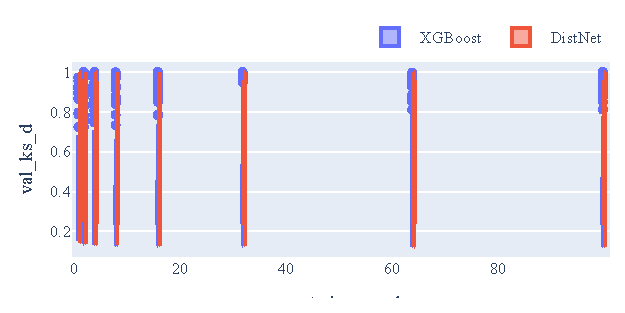
\includegraphics[trim={3.7cm 3.7cm 2.4cm 0},clip]{figures/10/figures/performances/legend.pdf}
%         \caption{Caption}
%     \end{subfigure}
%     \caption{NLLH}
%     \label{fig:placeholder}
% \end{figure*}


% \begin{figure}
%     \centering
%     % \begin{subfigure}{0.195\linewidth}
%     %     \includegraphics[width=\linewidth]{figures/10/figures/performances/clasp_factoring_lognorm_cpu_training_time_vs_obs.pdf}
%     %     \caption{Caption}
%     % \end{subfigure}
%     \begin{subfigure}{0.49\linewidth}
%         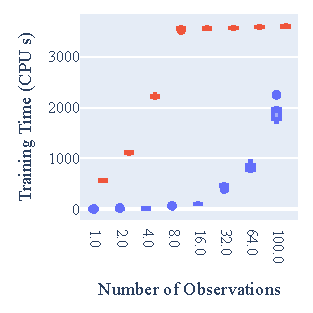
\includegraphics[width=0.8\linewidth]{figures/10/figures/performances/saps-CVVAR_lognorm_cpu_training_time_vs_obs.pdf}
%         \caption{Caption}
%     \end{subfigure}
%     % \begin{subfigure}{0.195\linewidth}
%     %     \includegraphics[width=\linewidth]{figures/10/figures/performances/spear_qcp_lognorm_cpu_training_time_vs_obs.pdf}
%     %     \caption{Caption}
%     % \end{subfigure}
%     % \begin{subfigure}{0.195\linewidth}
%     %     \includegraphics[width=\linewidth]{figures/10/figures/performances/yalsat_qcp_lognorm_cpu_training_time_vs_obs.pdf}
%     %     \caption{Caption}
%     % \end{subfigure}
%     % \begin{subfigure}{0.195\linewidth}
%     %     \includegraphics[width=\linewidth]{figures/10/figures/performances/spear_swgcp_lognorm_cpu_training_time_vs_obs.pdf}
%     %     \caption{Caption}
%     % \end{subfigure}
%     % \begin{subfigure}{0.195\linewidth}
%     %     \includegraphics[width=\linewidth]{figures/10/figures/performances/yalsat_swgcp_lognorm_cpu_training_time_vs_obs.pdf}
%     %     \caption{Caption}
%     % \end{subfigure}
%     \begin{subfigure}{0.49\linewidth}
%         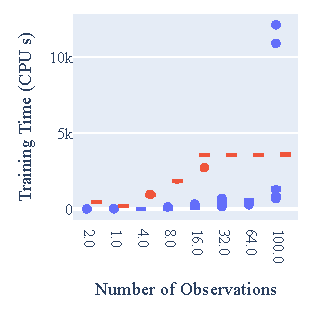
\includegraphics[width=0.8\linewidth]{figures/10/figures/performances/lpg-zeno_lognorm_cpu_training_time_vs_obs.pdf}
%         \caption{Caption}
%     \end{subfigure}

%     \begin{subfigure}{1.0\linewidth}
%     \centering
%         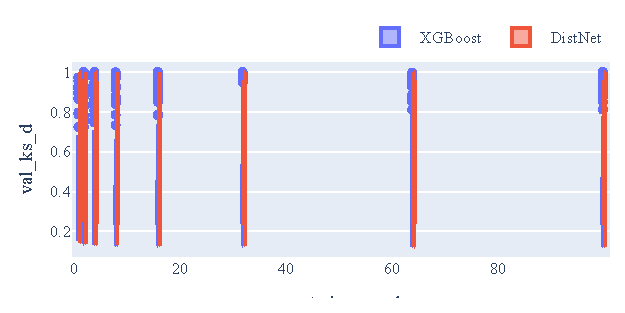
\includegraphics[trim={3.7cm 3.7cm 2.4cm 0.9cm},clip]{figures/10/figures/performances/legend.pdf}
%         % \caption{Caption}
%     \end{subfigure}
%     \caption{Time}
%     \label{fig:cpu_training_time}
% \end{figure}

\begin{figure}[htbp]
    \centering
    \begin{subfigure}{0.3\linewidth}
        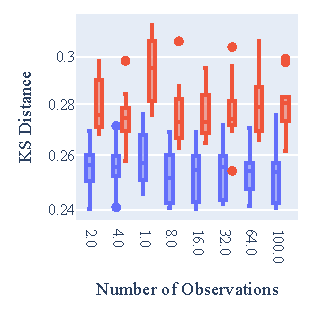
\includegraphics[]{figures/10/figures/performances/clasp_factoring_lognorm_val_ks_d_vs_obs.pdf}
        \caption{Clasp-Factoring}
        \label{fig:clasp_factoring_ks_d_vs_obs}
    \end{subfigure}
    \begin{subfigure}{0.3\linewidth}
        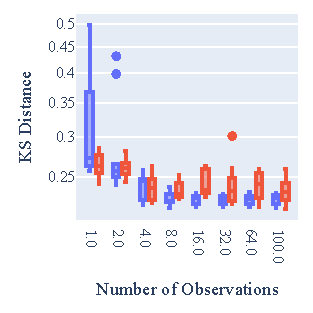
\includegraphics[]{figures/10/figures/performances/saps-CVVAR_lognorm_val_ks_d_vs_obs.pdf}
        \caption{Saps-CV-VAR}
        \label{fig:saps_cvvar_ks_d_vs_obs}
    \end{subfigure}
    \begin{subfigure}{0.3\linewidth}
        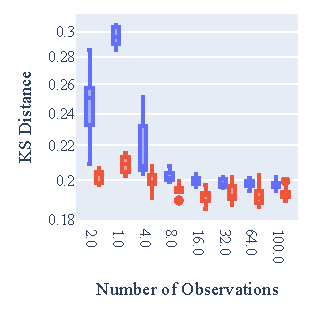
\includegraphics[]{figures/10/figures/performances/spear_qcp_lognorm_val_ks_d_vs_obs.pdf}
        \caption{Spear-QCP}
        \label{fig:spear_qcp_ks_d_vs_obs}
    \end{subfigure}
    \begin{subfigure}{0.3\linewidth}
        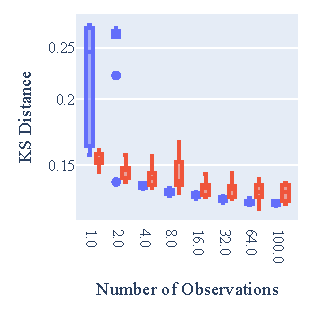
\includegraphics[]{figures/10/figures/performances/yalsat_qcp_lognorm_val_ks_d_vs_obs.pdf}
        \caption{YalSAT-QCP}
        \label{fig:yalsat_qcp_ks_d_vs_obs}
    \end{subfigure}
    \begin{subfigure}{0.3\linewidth}
        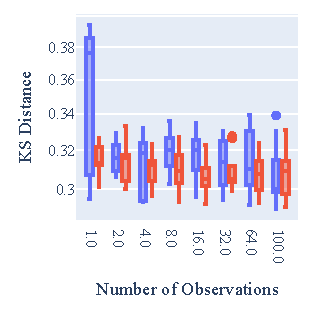
\includegraphics[]{figures/10/figures/performances/spear_swgcp_lognorm_val_ks_d_vs_obs.pdf}
        \caption{Spear-SWGCP}
        \label{fig:spear_swgcp_ks_d_vs_obs}
    \end{subfigure}
    \begin{subfigure}{0.3\linewidth}
        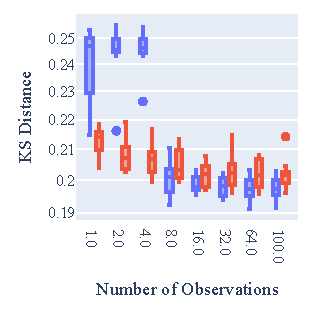
\includegraphics[]{figures/10/figures/performances/yalsat_swgcp_lognorm_val_ks_d_vs_obs.pdf}
        \caption{YalSAT-SWGCP}
        \label{fig:yalsat_swgcp_ks_d_vs_obs}
    \end{subfigure}
    \begin{subfigure}{0.3\linewidth}
        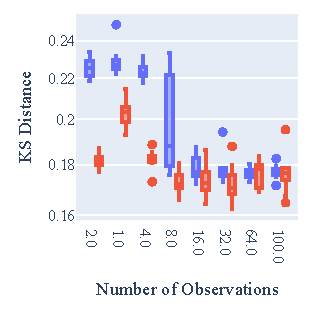
\includegraphics[]{figures/10/figures/performances/lpg-zeno_lognorm_val_ks_d_vs_obs.pdf}
        \caption{LPG-Zenotravel}
        \label{fig:lpg_zeno_ks_d_vs_obs}
    \end{subfigure}
    \begin{subfigure}{0.3\linewidth}
        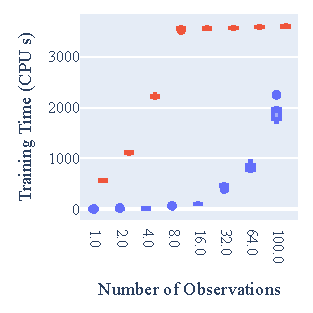
\includegraphics[]{figures/10/figures/performances/saps-CVVAR_lognorm_cpu_training_time_vs_obs.pdf}
        \caption{Saps-CV-VAR (time)}
        \label{fig:saps_cvvar_cpu_training_time_vs_obs}
    \end{subfigure}
    \begin{subfigure}{0.3\linewidth}
        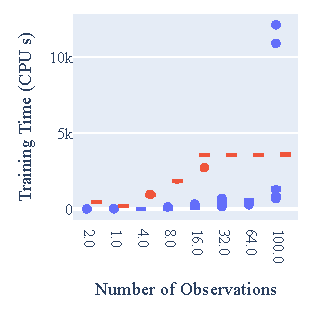
\includegraphics[]{figures/10/figures/performances/lpg-zeno_lognorm_cpu_training_time_vs_obs.pdf}
        \caption{LPG-Zenotravel (time)}
        \label{fig:lpg_zeno_cpu_training_time_vs_obs}
    \end{subfigure}
    
    \begin{subfigure}{1.0\linewidth}
    \centering
        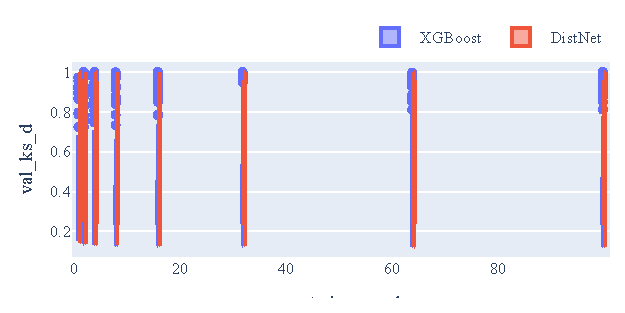
\includegraphics[trim={6.2cm 4.3cm 0cm 0.0cm},clip]{figures/10/figures/performances/legend.pdf}
        % \caption{Caption}
    \end{subfigure}
    \caption{Prediction quality and training efficiency of XGBoost \emph{vs} DistNet. (a--g) KS distance between predicted and observed running time distributions as a function of the number of training observations per instance, across seven scenarios, predicting the parameters of a \emph{log-normal} distribution; lower is better. XGBoost (blue) performs on par with DistNet (red) across all scenarios, with notable exceptions in the low-data regime, where DistNet retains a performance edge. Both methods improve with more observations added. (h--i) CPU training time comparison on one SAT and one automated planning scenario. XGBoost requires orders of magnitude less 
    % \hh{slightly modified:}
    computation (running time) than DistNet while achieving competitive prediction quality. 
    % \hh{I would swap subfigures h and i, for consistency with the order in which they appear earlier.}
    }
    \label{fig:genperf}
\end{figure}
\FloatBarrier


\subsection{Explainability analysis in SAT: Spear-SWGCP}

% \hh{I find the text in the plots way too small, but we can probably wait until preparing the CRC to improve this. let's not forget about it, though.}

% \hh{I would start differently here, reiterating (very briefly) what the goals are, in general terms -- i.e., why would one care about the analysis that follow? it would also be good to mention somewhere (earlier) why the two specific scenarios were chosem for explainability analysis presented here.}
% Through the newly introduced explainability perspective,
% we first look at one selected SAT solving scenario.
We analyse the running time distribution of the Spear SAT solver on the Small World Graph Colouring Problem (SWGCP)~\citep{GenEtAl99} instances using SATZilla features~\citep{HutEtAl14,ShaHoo24}.
Figures~\ref{fig:spear_swgcp_permut} and~\ref{fig:spear_swgcp_ice} show permutation importance rankings per statistic and ICE curves for the top feature per statistic, respectively.
The results reveal a clear structure: the most influential features for the scale statistics (mean, variance and IQR) are local-search probing features, while DPLL probing features are the most influential for the shape statistics (skewness and kurtosis).

\begin{figure}[!tbp]
    \centering
    % --- Spear-SWGCP: permutation importance ---
    \begin{subfigure}{0.3\linewidth}
        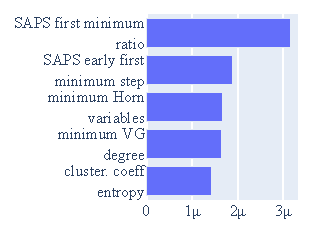
\includegraphics{figures/10/figures/explainability/spear_swgcp_xgb_dist_lognorm_100_fold0_mean_permutation_importance.pdf}
        \caption{Mean}
        \label{fig:spear_swgcp_mean_permutation_importance}
    \end{subfigure}
    \begin{subfigure}{0.3\linewidth}
        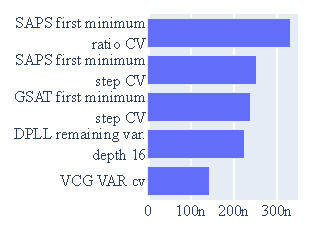
\includegraphics{figures/10/figures/explainability/spear_swgcp_xgb_dist_lognorm_100_fold0_variance_permutation_importance.pdf}
        \caption{Variance}
        \label{fig:spear_swgcp_variance_permutation_importance}
    \end{subfigure}
    \begin{subfigure}{0.3\linewidth}
        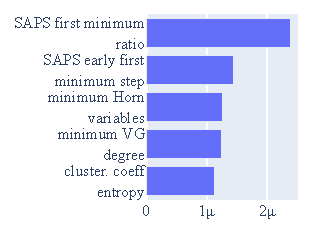
\includegraphics{figures/10/figures/explainability/spear_swgcp_xgb_dist_lognorm_100_fold0_iqr_permutation_importance.pdf}
        \caption{IQR}
        \label{fig:spear_swgcp_iqr_permutation_importance}
    \end{subfigure}
    \begin{subfigure}{0.3\linewidth}
        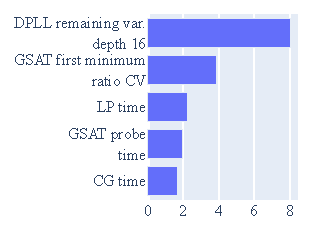
\includegraphics{figures/10/figures/explainability/spear_swgcp_xgb_dist_lognorm_100_fold0_skewness_permutation_importance.pdf}
        \caption{Skewness}
        \label{fig:spear_swgcp_skewness_permutation_importance}
    \end{subfigure}
    \begin{subfigure}{0.3\linewidth}
        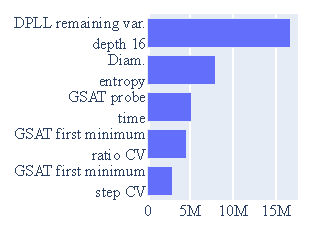
\includegraphics{figures/10/figures/explainability/spear_swgcp_xgb_dist_lognorm_100_fold0_kurtosis_permutation_importance.pdf}
        \caption{Kurtosis}
        \label{fig:spear_swgcp_kurtosis_permutation_importance}
    \end{subfigure}
    \caption{Permutation importance rankings for the predicted running time distribution statistics of Spear on SWGCP. Mean and IQR are dominated by SAPS local-search probing features, variance by the variability of the same probing signal, and skewness and kurtosis by the number of variables remaining after depth-16 unit-propagation probing.}
    \label{fig:spear_swgcp_permut}
\end{figure}

For mean and IQR, the most influential feature is the mean ratio of the first local minimum value to the starting value during a short SAPS~\citep{HutEtAl02} local-search run.
SAPS aims to minimise the number of unsatisfied clauses; therefore, a ratio near 1 means that the first local minimum has an objective value close to the initial one, while a lower value would indicate stronger early improvement.
The ICE curves show a small step increase in predicted mean and IQR as the ratio moves from approximately 1.0 to 1.06, and the effect is essentially flat for larger values, including the region above 1.1.
This suggests that once early SAPS probing fails to improve beyond the starting objective, the predicted running time and IQR of Spear move to a higher but stable regime.
For prediction of variance, the coefficient of variation of the first local minimum ratio is the most influential feature, with higher variability in local search behaviour across different runs translating to higher variance of the overall running time distribution.
This effect appears early in the observed feature range and then plateaus, suggesting that even moderate instability in the probing signal is enough to identify instances with more variable Spear running times.

Skewness and kurtosis are instead most influenced by the fraction of variables remaining after unit propagation at depth 16 in DPLL probing, capturing residual formula complexity after simplification rather than local search dynamics.
The corresponding ICE curves exhibit stronger instance-level heterogeneity than the mean, variance and IQR SAPS features.
Skewness is highest for intermediate fractions of remaining variables, whereas kurtosis decreases substantially as more variables remain after probing.


\begin{figure}[!tbp]
    \centering
    % --- Spear-SWGCP: ICE ---
    \begin{subfigure}{0.3\linewidth}
        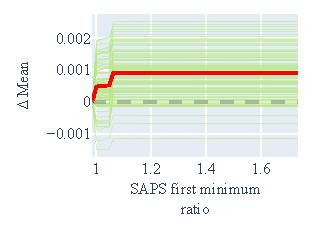
\includegraphics{figures/10/figures/explainability/spear_swgcp_xgb_dist_lognorm_100_fold0_mean_ice_feature59.pdf}
        \caption{Mean }
        \label{fig:spear_swgcp_mean_ice}
    \end{subfigure}
    \begin{subfigure}{0.3\linewidth}
        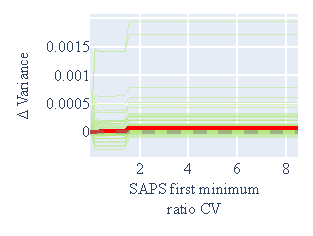
\includegraphics{figures/10/figures/explainability/spear_swgcp_xgb_dist_lognorm_100_fold0_variance_ice_feature60.pdf}
        \caption{\footnotesize Variance}
        \label{fig:spear_swgcp_variance_ice}
    \end{subfigure}
    \begin{subfigure}{0.3\linewidth}
        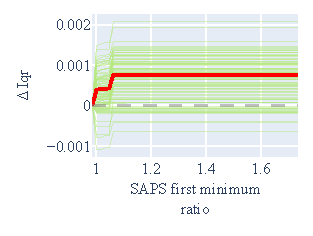
\includegraphics{figures/10/figures/explainability/spear_swgcp_xgb_dist_lognorm_100_fold0_iqr_ice_feature59.pdf}
        \caption{\footnotesize IQR}
        \label{fig:spear_swgcp_iqr_ice}
    \end{subfigure}
    \begin{subfigure}{0.3\linewidth}
        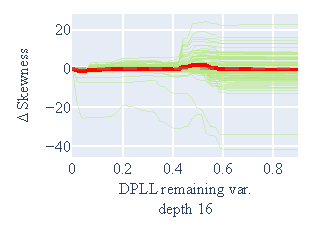
\includegraphics{figures/10/figures/explainability/spear_swgcp_xgb_dist_lognorm_100_fold0_skewness_ice_feature46.pdf}
        \caption{\footnotesize Skewness}
        \label{fig:spear_swgcp_skewness_ice}
    \end{subfigure}
    \begin{subfigure}{0.3\linewidth}
        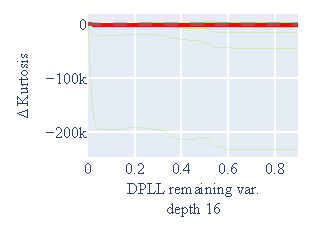
\includegraphics{figures/10/figures/explainability/spear_swgcp_xgb_dist_lognorm_100_fold0_kurtosis_ice_feature46.pdf}
        \caption{Kurtosis}
        \label{fig:spear_swgcp_kurtosis_ice}
    \end{subfigure}
    \caption{Centred ICE curves for the most important feature of each predicted statistic for Spear on SWGCP. Green curves show individual instances and red curves show partial dependence. The scale statistics change mostly through SAPS first-local-minimum features, while the shape statistics are more heterogeneous and depend on the residual formula size after unit propagation.}
    \label{fig:spear_swgcp_ice}
\end{figure}
\FloatBarrier
% Other highly ranked features for the mean and IQR include the clustering coefficient entropy of the variable-clause graph and the minimum Horn variable frequency.
% This indicates that both local search dynamics and problem structure contribute to central tendency of the running time distribution in this scenario.
% \hh{very nicely  summarised!}
% \aj{In the following it seems that we refer to all subfigures whereas in reality we talk only about mean and IQR here, so I would change accordingly}
% For prediction of the mean, the permutation importance rankings show that the most influential feature is the mean ratio of the first local minimum value to the starting value during local search probing (Figure~\ref{fig:spear_swgcp_mean_permutation_importance}).
% The permutation importance rankings in Figures~\ref{fig:spear_swgcp_mean_permutation_importance}--\ref{fig:spear_swgcp_kurtosis_permutation_importance} show that the most important feature for mean prediction is the mean ratio of the first local minimum value to the starting value during local search probing (Figure~\ref{fig:spear_swgcp_mean_permutation_importance}). 
% This feature, which also ranks highest for IQR (Figure~\ref{fig:spear_swgcp_iqr_permutation_importance}), measures how quickly local search algorithms reach their first local minimum relative to their starting point. Other highly ranked features for the mean and IQR include the clustering coefficient entropy of the variable-clause graph and the minimum Horn variable frequency.
% This indicates that both local search dynamics and problem structure contribute to central tendency 
% % \hh{added:}
% of the running time distribution of the Spear solver.

% The ICE curves for the mean and IQR (Figures~\ref{fig:spear_swgcp_mean_ice} and~\ref{fig:spear_swgcp_iqr_ice}) reveal a
% threshold effect, whereby the predicted statistics remain relatively stable until the first local minimum ratio reaches approximately 1.0, after which there is a sharp increase. 
% This discontinuity suggests that instances where local search quickly reaches a plateau (ratio close to 1) represent a fundamentally different computational regime than instances requiring more exploration to reach the first local minimum. 
% The clustering of individual ICE curves around the partial dependence line indicates that this effect is consistent across instances, with little interaction with other features.

% For variance prediction (Figure~\ref{fig:spear_swgcp_variance_permutation_importance}), the coefficient of variation of the first local minimum ratio emerges as the most influential feature, followed by the coefficient of variation of the first local minimum step and the fraction of variables reduced at depth 16. A higher coefficient of variation indicates that the local search behaviour is inconsistent across different runs. The ICE curve for variance (Figure~\ref{fig:spear_swgcp_variance_ice}) shows that higher variability in reaching the first local minimum translates into higher variance of the overall running time distribution, with the relationship becoming more pronounced for feature values between 1.5 and 2.0. This suggests a critical threshold beyond which solver performance becomes highly unstable, which is useful for identifying instances that may require multiple restarts or alternative solving strategies.

% The higher-order moments exhibit a different feature importance profile. Both skewness and kurtosis (Figures~\ref{fig:spear_swgcp_skewness_permutation_importance} and~\ref{fig:spear_swgcp_kurtosis_permutation_importance}) are primarily influenced by the fraction of variables that remain after unit propagation at depth 16 in the search tree, with the diameter entropy of the variable-clause graph also ranking highly for kurtosis. These features capture the structural complexity of the instance after initial simplification rather than local search dynamics. The ICE curves for skewness and kurtosis (Figures~\ref{fig:spear_swgcp_skewness_ice} and~\ref{fig:spear_swgcp_kurtosis_ice}) reveal a qualitatively different pattern: while the average partial dependence (shown by the red line) is relatively flat across the feature range, individual instance curves exhibit extreme sensitivity, with large positive and negative deviations concentrated in the 0.4 to 0.6 range. This heterogeneous behaviour indicates strong interaction effects with other instance features; instances that retain a moderate fraction of variables after depth-16 propagation can exhibit either very symmetric or very heavy-tailed running time distributions, depending on other structural characteristics such as the variable-clause graph topology.
% The separation between features driving scale statistics (mean, variance, IQR) and shape statistics (skewness, kurtosis) provides useful insights for practitioners in SAT solving and closely related domains. 
% \aj{rephrase the following until the end of paragraph to lose the gemini vibe, proposal below}
% Those seeking to identify instances with predictable running times \aj{what does predictable running times even mean here? Of course we are interested in those instances, no? Ideally all instances will have predictable running times, i.e., running times that can be predicted. What could we say instead? How can we replace this?} should focus on local search probing features, particularly the first local minimum ratio and its variability. In contrast, those concerned about tail risk, such as the potential for occasional extreme outliers that could violate time budgets, should examine the residual problem complexity after unit propagation. The fact that different features dominate different aspects of the distribution suggests that instance hardness is multifaceted: an instance may have moderate expected running time but high tail risk, or vice versa, and these characteristics are driven by distinct structural properties.


\subsection{Explainability analysis in automated planning: LPG-Zenotravel}
% We now shift our attention to a scenario from the automated planning domain. 
We analyse the running time distribution of the LPG stochastic local search planner~\citep{GerSer02} on the Zenotravel~\citep{PenWel94} instances.
Figures~\ref{fig:lpg_zeno_permut} and~\ref{fig:lpg_zeno_ice} show permutation importance rankings per statistic and ICE curves for the top feature per statistic, respectively.
The planning feature set combines planning-native descriptors, such as PDDL, causal-graph, domain-transition-graph and probing features, with SAT features obtained by translating the planning task into a bounded-horizon CNF representation~\citep{FawEtAl14}.
In this scenario, the scale statistics (mean, variance, IQR) are driven mainly by features of this SAT encoding, whereas the shape statistics (skewness, kurtosis) are driven by a planning-native domain-transition-graph feature.

\begin{figure}[!tbp]
    \centering
    % --- LPG-Zenotravel: permutation importance ---
    \begin{subfigure}{0.3\linewidth}
        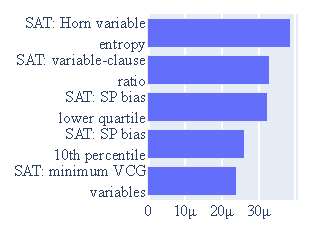
\includegraphics{figures/10/figures/explainability/lpg-zeno_xgb_dist_lognorm_100_fold0_mean_permutation_importance.pdf}
        \caption{Mean}
        \label{fig:lpg_zeno_mean_permutation_importance}
    \end{subfigure}
    \begin{subfigure}{0.3\linewidth}
        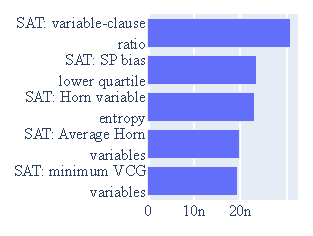
\includegraphics{figures/10/figures/explainability/lpg-zeno_xgb_dist_lognorm_100_fold0_variance_permutation_importance.pdf}
        \caption{Variance}
        \label{fig:lpg_zeno_variance_permutation_importance}
    \end{subfigure}
    \begin{subfigure}{0.3\linewidth}
        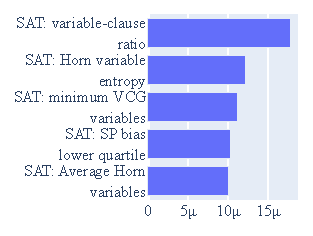
\includegraphics{figures/10/figures/explainability/lpg-zeno_xgb_dist_lognorm_100_fold0_iqr_permutation_importance.pdf}
        \caption{IQR}
        \label{fig:lpg_zeno_iqr_permutation_importance}
    \end{subfigure}
    \begin{subfigure}{0.3\linewidth}
        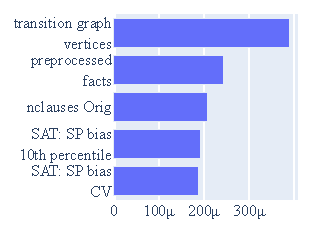
\includegraphics{figures/10/figures/explainability/lpg-zeno_xgb_dist_lognorm_100_fold0_skewness_permutation_importance.pdf}
        \caption{Skewness}
        \label{fig:lpg_zeno_skewness_permutation_importance}
    \end{subfigure}
    \begin{subfigure}{0.3\linewidth}
        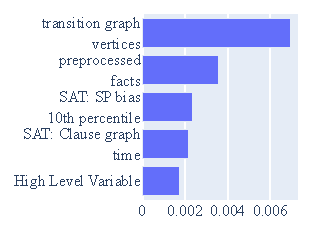
\includegraphics{figures/10/figures/explainability/lpg-zeno_xgb_dist_lognorm_100_fold0_kurtosis_permutation_importance.pdf}
        \caption{Kurtosis}
        \label{fig:lpg_zeno_kurtosis_permutation_importance}
    \end{subfigure}

    \caption{Permutation importance rankings for the predicted running time distribution statistics of LPG on Zenotravel. The scale statistics are mainly driven by SAT-encoding features extracted from the planning task, while skewness and kurtosis are dominated by the size of the planning domain-transition graph.}
    \label{fig:lpg_zeno_permut}
\end{figure}

For predictions of mean running time, the most influential feature is the entropy of the distribution of Horn-clause variable occurrences in the SAT encoding.
The proximity-to-Horn features summarise how close the encoded formula is to Horn structure by measuring, for each variable, its occurrence in Horn clauses.
High entropy indicates that this Horn-related structure is spread more uniformly across variables in the bounded planning encoding.
The corresponding ICE curve shows only a small average effect, but predicted mean running time increases toward the high end of the observed entropy range.
Other highly ranked mean features include the SAT variable-to-clause ratio and survey-propagation bias features, indicating that central tendency is explained mostly by the constraint structure of the SAT representation rather than by a single PDDL-size feature.

For variance and IQR, the top feature is the variable-to-clause ratio of the SAT encoding.
This ratio is a simple structural measure of the encoded CNF: over the observed Zenotravel instances, larger values correspond to fewer clauses per variable and hence lower clause density.
The ICE curves for variance and IQR are monotonic over the observed range, with both predicted statistics increasing as the variable-to-clause ratio grows.
Thus, the spread of LPG runtimes is associated with how the planning instance is represented as a propositional constraint problem.

Skewness and kurtosis exhibit a different behaviour.
Both skewness and kurtosis are primarily influenced by the total number of vertices in the domain transition graphs, a planning-native feature.
Domain transition graphs describe the possible value transitions of finite-domain planning variables. Their total number of vertices reflects the aggregate size of these variable domains.
The ICE curves show increasing skewness and kurtosis as this transition structure grows, with the strongest increase near the upper end of the observed range.
This suggests that tail behaviour for LPG-Zenotravel is tied to the size of the underlying finite-domain transition structure, while mean and dispersion are tied more strongly to the bounded SAT encoding used by the feature extractor.


\begin{figure}[!tbp]
    \centering
    % --- LPG-Zenotravel: ICE ---
    \begin{subfigure}{0.3\linewidth}
        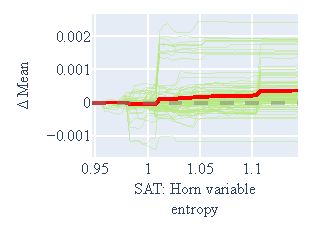
\includegraphics{figures/10/figures/explainability/lpg-zeno_xgb_dist_lognorm_100_fold0_mean_ice_feature2.pdf}
        \caption{Mean}
        \label{fig:lpg_zeno_mean_ice}
    \end{subfigure}
    \begin{subfigure}{0.3\linewidth}
        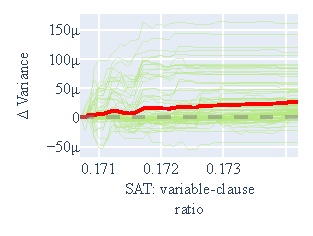
\includegraphics{figures/10/figures/explainability/lpg-zeno_xgb_dist_lognorm_100_fold0_variance_ice_feature62.pdf}
        \caption{Variance}
        \label{fig:lpg_zeno_variance_ice}
    \end{subfigure}
    \begin{subfigure}{0.3\linewidth}
        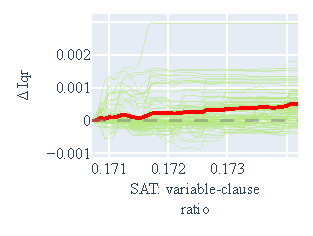
\includegraphics{figures/10/figures/explainability/lpg-zeno_xgb_dist_lognorm_100_fold0_iqr_ice_feature62.pdf}
        \caption{IQR }
        \label{fig:lpg_zeno_iqr_ice}
    \end{subfigure}
    \begin{subfigure}{0.3\linewidth}
        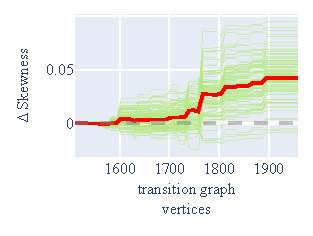
\includegraphics{figures/10/figures/explainability/lpg-zeno_xgb_dist_lognorm_100_fold0_skewness_ice_feature135.pdf}
        \caption{Skewness}
        \label{fig:lpg_zeno_skewness_ice}
    \end{subfigure}
    \begin{subfigure}{0.3\linewidth}
        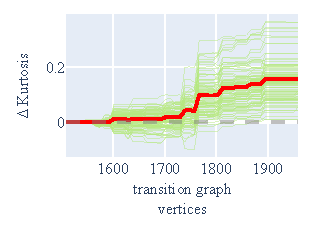
\includegraphics{figures/10/figures/explainability/lpg-zeno_xgb_dist_lognorm_100_fold0_kurtosis_ice_feature135.pdf}
        \caption{Kurtosis}
        \label{fig:lpg_zeno_kurtosis_ice}
    \end{subfigure}


    \caption{Centred ICE curves for the most important feature of each predicted statistic for LPG on Zenotravel. Green curves show individual instances and red curves show partial dependence. Horn-variable entropy in the SAT encoding affect mean running time, the SAT variable-to-clause ratio governs variance and IQR, and the number of domain-transition-graph vertices affect skewness and kurtosis.}
    \label{fig:lpg_zeno_ice}
\end{figure}
\FloatBarrier




\section{Conclusions and future work}
\label{sec:concl}

In this work, we proposed a methodology for explaining distribution predictions, in the context of algorithm running time distributions. To this end, we used a probabilistic XGBoost which offers a computationally efficient and stable alternative to neural network approaches. Our explanation framework decomposes predicted distributions into interpretable scale and shape statistics, allowing the application of permutation importance and ICE curves to analyse how specific features influence different aspects of solver performance.

Our empirical analysis on SAT solving and automated planning yields concrete, insights for researchers. Specifically, we demonstrated that:
In SAT solving (specifically, the Spear solver on SWGCP instances), scale statistics (mean and variance) are influenced by early local-search probing dynamics, while shape statistics (skewness and kurtosis) are affected more by DPLL-simplification features. 
In automated planning (LPG planner on Zenotravel instances), scale statistics are explained by SAT-encoding characteristics, whereas tail risks are impacted by planning-native domain transition graph sizes. 

Our work can be extended in several directions. Firstly, performance distribution prediction has been applied only to running time data of solvers for $\mathcal{NP}$-complete problems. In the future, it is possible to study the performance distributions of additional algorithms for fundamentally different problems, such as machine learning (\emph{e.g.}, training time or hyperparameter tuning stability of deep neural networks). Additionally, while XGBoost matched the predictive quality of DistNet, there remains a gap in modelling low-data regimes (1–8 observations per instance), where neural network approaches still hold a performance edge. Future research can focus on bridging this gap by exploring tree-based architectures with probabilistic priors or hybrid neural-tree models that maintain high explainability without compromising data efficiency.

Overall, we believe that performance of randomised algorithms should not be evaluated and explained based on single statistics, such as the mean, but on the full distribution, to better understand the full range of algorithm behaviour.}